%!TEX root = ../report.tex
\section{Divergence}
\label{sec:divergence}
Divergence shows how much fluid is sucked into a sink or pulled out of a source. 
Calculation of divergence is done by taking the derivatives of vector fields, which results in a scalar value.
Taking the derivative of a vector field can be approximated by using differences.
We decided to use the central difference in the $x$-direction, as well as in the $y$-direction, since this will yield the most stable outcome.
The function has the following dimensions:  $f:\mathbb{R}^2 \rightarrow \mathbb{R}^1$.
So once the divergence is computed, it is just a matter of colormapping the scalar value as in Section~\ref{sec:color_mapping}.

Divergence at point $p_{x,y}$ can be calculated using a couple of steps:

\begin{equation*}
\begin{aligned}
\nabla d &= \Delta x + \Delta y \\
\Delta x &= p_{x+1,y} - p_{x-1,y} \\
\Delta y &= p_{x,y+1} - p_{x,y-1} \\
\end{aligned}
\end{equation*}

Divergence in action can be seen in Figure~\ref{fig:div_velo}.
\begin{figure}[htb]
    \centering
    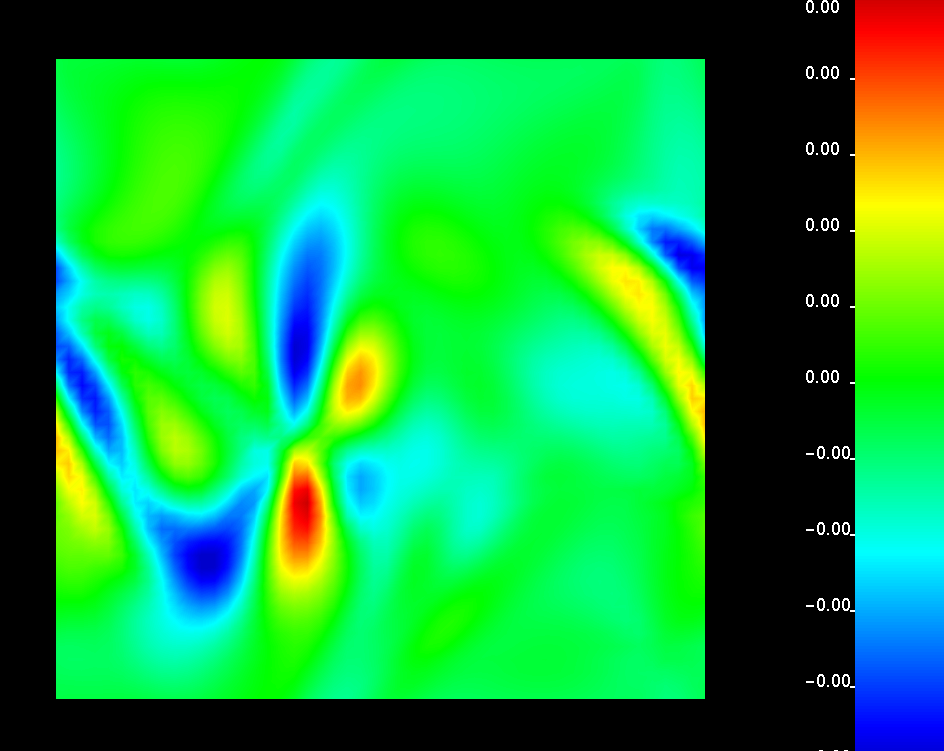
\includegraphics[width =0.5\textwidth]{content/pictures/div_velo.png}
    \caption{Divergence of the velocity field}
    \label{fig:div_velo}
\end{figure}

In Figure~\ref{fig:force_field}, it can be observed that there is a high correlation between the magnitude of the force field $||\vec{F}||$ in Figure~\ref{fig:force_mag} and the divergence of this field $\nabla \vec{F}$ in Figure~\ref{fig:div_force}.
The reason that these two visualizations are very similar is due to the simulation of the model: The model itself has no fixed sources or sinks. 
When the mouse is clicked, a source created at that location, so sources exist on the positions where a force is present.
\begin{figure}[htb]
    \centering
    \begin{subfigure}[htb]{.49\textwidth}
        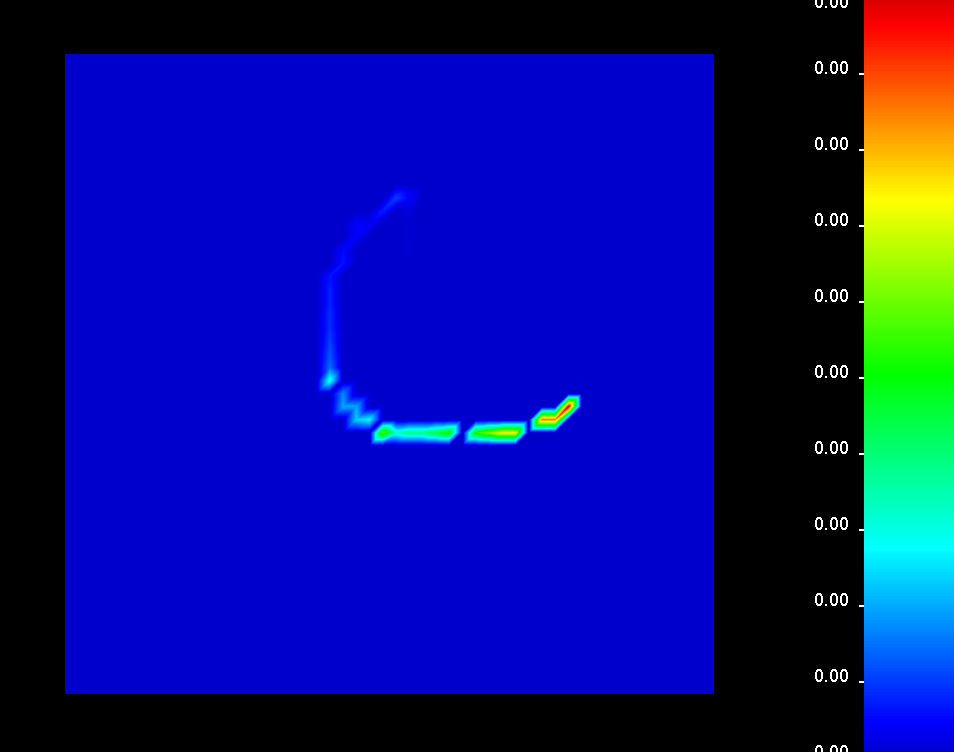
\includegraphics[width =\textwidth]{content/pictures/force_magnitude.png}
        \caption{Magnitude of force field ($||f||$)}
        \label{fig:force_mag}
    \end{subfigure}
    \begin{subfigure}[htb]{.49\textwidth}
        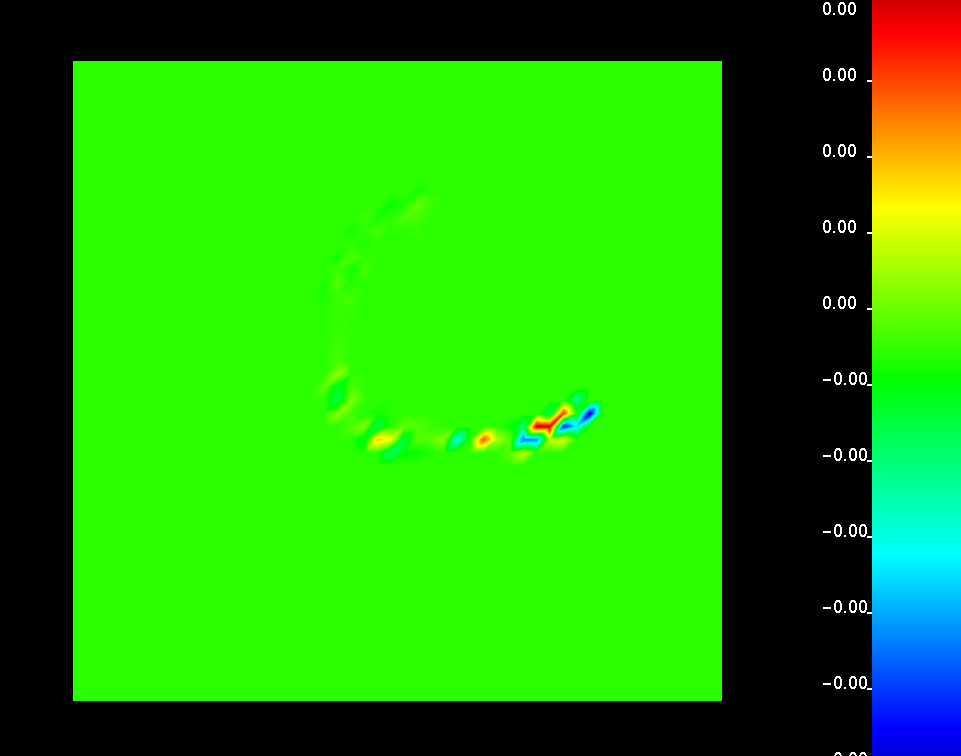
\includegraphics[width =\textwidth]{content/pictures/div_force.png}
        \caption{Divergence of force field ($\nabla f$) }
        \label{fig:div_force}
    \end{subfigure}
    \caption{Force field visualization}
    \label{fig:force_field}
\end{figure}


\clearpage